\clearpage
\section{相关理论研究基础}
\subsection{流行病动力学中的基本概念}
为了接下来的模型介绍,这部分要阐述流行病动力学中的几个重要基本概念,并解释他们的现实意义。

设病人受到感染是与他人接触造成的,单位时间内一个病人与其他人接触的次数称为接触率,接触率通常依赖于总人口$N$,如果被接触者为易感者,那么就会有一定的概率收到感染,设每次接触收到传染的概率为$\beta$,把$\beta$称为有效接触率(effective contact rate)。指的是在接触的人群中,有多少人是易感人群,即患病的概率较高的人。在疫情流行期间,有效接触率是一个重要的参数,因为它直接影响到疾病传播速度和规模的大小。如果有效接触率过高,就意味着病毒传播的速度也会更快,从而导致更多的人感染。

由于易感者在总人口中的比例为$\frac{S}{N}$,因此每一个病人的有效接触率为$\beta N \frac{S}{N}$,也就是每个病人对易感者的平均感染率(average infection rate),指的是在一个特定的时间段内,一个感染病毒的人平均会传染给多少其他人。它是流行病学中一个重要的指标,用来描述疾病传播的速度和强度。平均感染率通常由多个因素决定,包括病原体的传播能力、人群的易感性和接触模式等。在疫情控制和防控策略制定中,了解平均感染率是非常重要的。一旦确定了平均感染率,就可以采取相应的控制措施,例如隔离感染者、提高社交距离等,以减缓疾病传播速度,控制疫情规模。而单位时间内被感染的人数为
$$\beta N \frac{S(t)}{N(t)} I(t)$$

称为发生率。

为了区分疾病是否会长期流行,我们称
$$R_0=\frac{\beta N}{\gamma}$$

为基本再生数(basic reproduction number,简称$R_0$)是流行病学中用来描述一个传染病在人群中传播的能力的重要参数。它表示在一个人群中,一个感染病毒的人平均会传染给多少个易感人群。如果$R_0$大于1,就意味着疾病在人群中会持续传播,导致疫情扩大;如果$R_0$小于1,疾病会逐渐消失。$R_0$的大小通常受到多种因素的影响,包括病原体的传染性、人群的易感性、接触模式等。在疫情控制和防控策略制定中,了解$R_0$是非常重要的。一旦确定了$R_0$,就可以采取相应的控制措施,例如隔离感染者、提高社交距离等,以降低$R_0$,控制疫情规模。其中$\frac{1}{\gamma}$是病人的平均患病周期,基本再生数也表示平均一个病人在患病时感染的人数。一般来说,只有当易感者有补充时,例如有康复者失去免疫能力,再次获得感染能力;有出生、迁入等,才有可能产生地方病,即疾病在某个地区长期存在的情况。

平均一个病人在其感染期间内有效接触其他人的数量记作$\sigma$
$$\sigma=\beta N \frac{1}{\gamma}$$

$\sigma$称为(effective contact number,简称R)是流行病学中用来描述一个传染病在人群中传播的能力的指标之一。它表示每个感染者在传染期内平均接触到的易感人群数量,且这些接触者中有多少人最终会被感染。有效接触不一定会导致传染,只有对易感者的有效接触才会发生传染。

\subsection{SEIR模型}
\subsubsection{模型构建}
SEIR模型是一种常用的流行病学模型,用于描述人群中疾病的传播过程。这个模型将人群分为四类:易感者(S),潜伏者(E),感染者(I)和康复者(R),并考虑了潜伏期的存在。SEIR模型假设总人数不变,不考虑人口的迁入迁出和出生死亡。在这个模型中,病原体传播的过程是通过有效接触将易感者(S)转化为潜伏者(E)。然后,潜伏者(E)经过平均潜伏期后成为感染者(I)。感染者(I)可以被治愈并成为康复者(R),而康复者(R)则获得终身免疫,不再容易感染。这个模型的一个重要应用是预测疫情的发展趋势和估计疫情的控制措施效果。通过调整模型中的参数,我们可以评估不同控制措施对疫情的影响,从而制定出最优的控制策略。

\begin{gather}
\left\{
\begin{aligned}
\frac{dS}{dt} & =  -\frac{\beta SI}{N} \\
\frac{dE}{dt} & =  \frac{\beta SI}{N} - \alpha E\\
\frac{dI}{dt} & =  \alpha E - \gamma I \\
\frac{dR}{dt} & =  \gamma I \\
\end{aligned}
\right.
\label{equal:SEIR}
\end{gather}

其中日接触数 $\beta$ 为每个患病者每天有效接触的易感者的平均人数;日发病率 $\alpha$ 为每天发病成为患病者的潜伏者占潜伏者总数的比例;日治愈率 $\gamma$ 为每天被治愈的患病者人数占患病者总数的比例,即平均治愈天数为 $\frac{1}{\gamma}$。转换关系如下图\ref{img:SEIR}

\begin{figure}[htbp]
    \centering
    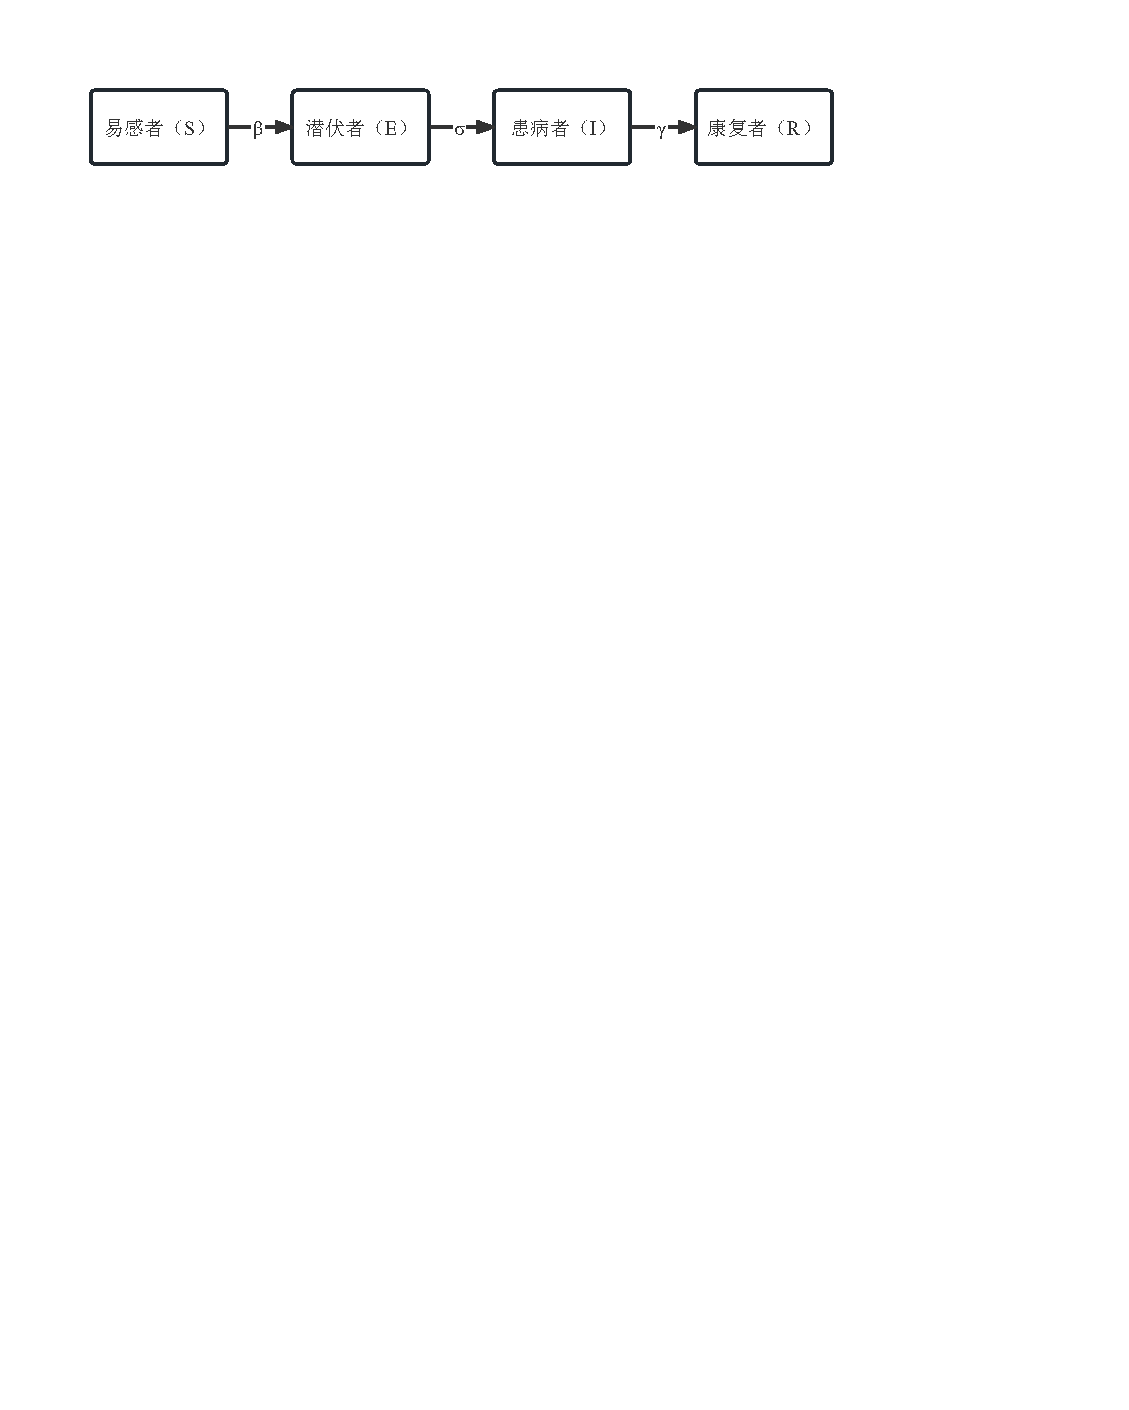
\includegraphics{image/SEIR}
    \caption{SEIR模型转换关系}
    \label{img:SEIR}
\end{figure} 

\subsubsection{稳定性理论}
常微分方程的稳定性理论是研究解的长期行为和稳定性的数学理论。在常微分方程中,稳定性理论通常用于分析动力系统的渐近行为,即研究当时间趋向于无穷大时,解的趋势和特性。

常微分方程的稳定性理论主要包括线性稳定性和非线性稳定性两个方面。线性稳定性理论主要适用于线性常微分方程,它通过研究方程解的增长率和其它特征来判断解的长期行为和稳定性。非线性稳定性理论则适用于非线性常微分方程,它通过研究方程解的奇异点、周期解、吸引子等来判断解的稳定性和演化趋势。

在应用中,常微分方程的稳定性理论可以用于分析各种动态系统,例如物理学中的振动系统、经济学中的供需模型、生物学中的种群动态模型等等。它不仅有助于理论研究,而且对于实际问题的求解和预测也有很大的帮助。

在SEIR模型中,稳定性理论可以用于分析该模型的长期行为和稳定性。具体来说,可以通过稳定性理论来研究以下问题:疫情的持续时间:利用稳定性理论可以判断疫情是否会在人群中持续传播,以及持续的时间有多长。疫情的规模:通过研究SEIR模型的长期行为和稳定性,可以预测疫情的最终规模和影响范围。干预措施的效果:稳定性理论可以帮助评估各种干预措施对疫情传播的控制效果,并找到最优策略。

当基本再生数$R_0$小于1时,SEIR模型的恢复者人数将最终趋于稳定,即疫情最终将消失。而当$R_0$大于1时,SEIR模型的感染者人数将保持稳定或增长,意味着疫情将在人群中持续传播。因此,稳定性理论可以用来预测疫情的持续时间和规模,并帮助评估不同干预措施的效果。

\begin{gather}
    R_0 = \beta  (\frac{1}{\gamma}+\frac{1}{\alpha})
\end{gather}

$R_0$对于制定疾病预防和控制策略至关重要,它可以帮助决策者了解疫情传播的趋势和规模,从而采取相应的干预措施。例如,如果$R_0$很高,政府可能会采取强制隔离、加强监测等措施来限制人员流动和传播;而如果$R_0$比较低,政府可能可以采取更为温和的干预措施,例如建立疫情监测系统和提醒公众做好防护措施等。此外,$R_0$还可以用来评估疫苗和药物的效果。通过研究疫苗或药物对$R_0$的影响,可以评估它们对疫情传播的控制效果和预防能力,为疫情防控提供科学依据。因此,基本再生数是研究疫情流行特征、制定防控策略和评估防疫药物和疫苗效果的重要指标。

\subsection{人工神经网络}
人工神经网络(ANN)是一种数学模型,其结构和功能仿照生物神经网络。它可以对函数进行估计或近似。神经网络由大量的人工神经元联结进行计算。这些神经元相互连接并通过不同的加权方式进行信号传递,从而形成一个复杂的网络结构。这个网络可以学习外界的信息,并自适应地改变内部结构,使得它能够具有学习和适应的能力。现代神经网络是一种非线性统计性数据建模工具,通过一个基于数学统计学类型的学习方法得以优化。这种学习方法使得神经网络能够发现和表达数据之间的复杂非线性关系,从而实现对复杂问题的建模和预测。在人工智能学的人工感知领域,我们可以通过数学统计学的应用来解决一些决策问题。与正式的逻辑学推理演算相比,神经网络的优势在于它能够模拟人类的简单决策和判断能力,从而更好地适应不同的任务和场景。因此,人工神经网络是一种强大的工具,可以在多个领域中得到广泛的应用,如医学诊断、金融预测、自然语言处理和图像识别等。其中,自然语言处理和图像识别是神经网络在人工智能领域中的两个重要应用方向。在自然语言处理中,神经网络可以用于文本分类、情感分析和机器翻译等任务。在图像识别中,神经网络可以用于物体检测、人脸识别和图像生成等任务。随着人工神经网络技术的不断发展和应用,它已成为现代计算机科学领域中不可或缺的一部分。而随着深度学习技术的兴起,神经网络已经成为解决大规模数据和复杂问题的重要工具,使得机器能够更好地模拟和理解人类的认知和行为。因此,人工神经网络是一种极具潜力的技术,它将在未来的人工智能领域中扮演着越来越重要的角色。

\subsubsection{网络构成}
人工神经元是人工神经网络的核心组成部分。每一个神经细胞从数个其它神经细胞那里得到信息,把这些信息与被赋予的权值相乘,再把这些信息相加,再把这些信息加到一个或更多的神经细胞上。有些人造神经细胞在向下一个变数传送输入量前,会先为该输入量设定一个激活函数。它的数学公式是这样的:

\begin{gather}
    t=f(\overrightarrow{W} \overrightarrow{A}+b)
\end{gather}

其中$\overrightarrow{W}$为权向量,$\overrightarrow{A}$为输入向量,$b$为偏置,$f$为激活函数。可见,一个神经元的功能是求得输入向量与权向量的内积后,经一个非线性传递函数得到一个标量结果。

一旦神经网络完成了对输入数据的计算,这些数据的值不会直接传递给下一层。相反,这些值需要经过一个激活函数的处理,以便在网络中进行学习并识别数据中的复杂模式。激活函数是一种添加到人工神经网络中的函数,其目的是在神经元中对输入数据进行处理,从而产生一个输出值。在神经网络中,每一层都是通过加权求和的方式进行输入输出的线性变换,没有激活函数的话,即使网络再复杂,多少层也无法解决更为复杂的问题。因此,激活函数的引入使得神经网络能够处理更广泛的非线性模型。此外,由于激活函数通常都是非线性的,因此我们在神经元中加入了一个非线性因素,使得神经网络能够近似任何其它的非线性函数。换句话说,激活函数的引入使得神经网络更加灵活和适应性强,能够更好地处理各种类型的问题,例如图像识别、语音识别、自然语言处理等等。

神经元网络是由若干个神经元构成的,每个神经元都接收相同的输入向量。每个神经元会输出一个标量结果,因此单层神经元的输出是一个向量,向量的维数等于神经元的数量。每一层都可以被看作是感知器,与上一层连接。然而,近年来出现了许多不同的深度神经网络架构,比如前馈神经网络、卷积神经网络、循环神经网络、长短期记忆和门循环单元。在这些网络中,前馈神经网络被广泛使用,因为它足以逼近最优控制函数。

前馈神经网络是感知器的集合,由输入层、隐藏层和输出层组成。在每个连接过程中,上一层的信号被乘以一个权重,增加一个偏置,然后通过一个激活函数。激活函数的引入使得神经网络可以学习数据中的非线性模式,从而可以处理更加复杂的问题。在前馈神经网络中,使用反向传播算法迭代更新权重和偏置参数,以优化网络性能。总之,虽然神经元网络最初是由有限个神经元构成,但现在已经发展成为了包含多种深度神经网络架构的复杂系统,这些网络可以通过学习逼近最优控制函数并处理更加复杂的问题。如图\ref{img:FNN}

\begin{figure}[htbp]
    \centering
    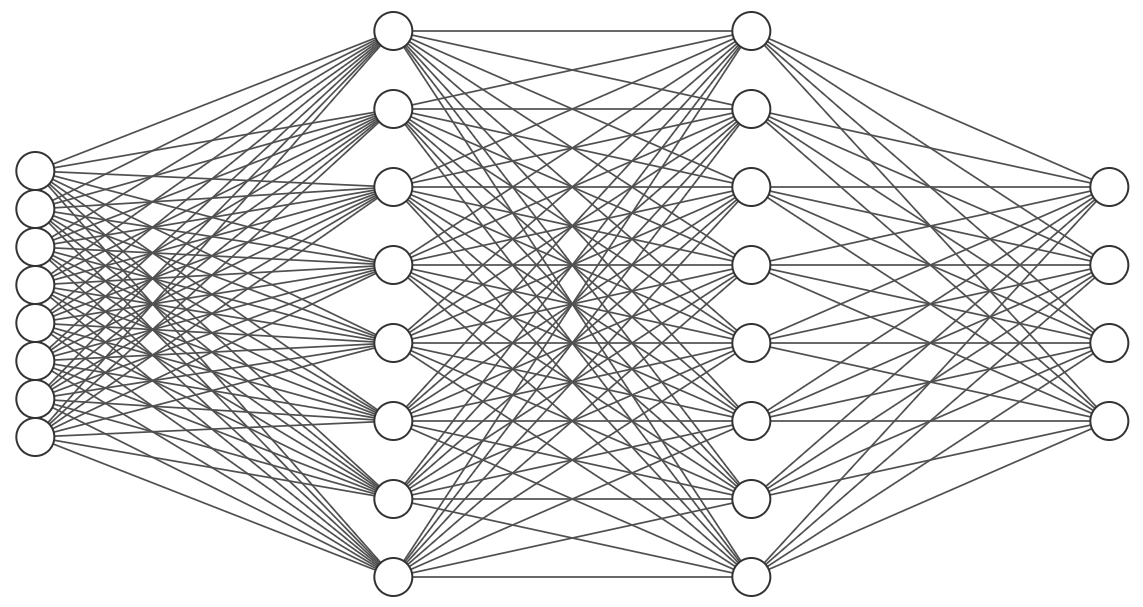
\includegraphics[width=0.8\linewidth]{image/NN}
    \caption{前馈网络}
    \label{img:FNN}
\end{figure} 

\subsubsection{网络优化}

万能近似定理\ucite{Pinkus1999ApproximationTO}表明:只需要使用需具备一个层隐含层和有限个神经单元的前馈神经网络,,就能以任意精度拟合任意复杂度的函数。万能逼近定理从理论上确保深度神经网络可以通过直接从数据中学习整个非线性交互集来逼近未知映射或算子。深度神经网络方法在实践中被证明可以很容易地找到好的参数来拟合数据或进行模型校准。更重要的是,好的参数不需要是唯一的,这意味着在实践中相信对于大型神经网络,局部最小值就足够了,而全局最小值往往会导致过度拟合。

人工神经网络是一种通过自动学习过程来对输入数据进行处理的算法。该算法通过对各个层的权重进行校正,以达到学习输入数据的目的。不同的网络结构和模型采用的学习方法也不尽相同,其中常用的一种是反向传播算法(Backpropagation)。在这个算法中,目标函数对各神经元权值的偏导数会被逐层计算出来,并构成了目标函数对权值向量的梯度。这个梯度会被用来修改神经网络中的参数,从而完成网络的学习。当网络输出的值与真实值的误差达到预期值时,网络的学习就会结束。

神经网络的优化算法有多种,下面是一些常见的:梯度下降(Gradient Descent):是一种基础的优化算法,通过计算目标函数的梯度,沿着梯度的方向更新参数值,使目标函数达到最小值。随机梯度下降(Stochastic Gradient Descent,SGD):是一种常用的梯度下降算法,与梯度下降相比,SGD每次只随机选择一个样本进行计算,更新参数。它可以减少计算量和内存占用,加快模型训练速度。动量(Momentum):是一种基于梯度的优化算法,通过加入动量项,使更新方向具有一定的惯性,避免模型在局部最小值处停留。自适应学习率(Adaptive Learning Rate):是一种自适应调整学习率的算法,如AdaGrad、Adam、RMSprop等。它们通过自适应地调整学习率,提高模型收敛速度和性能,避免学习率过大或过小导致的问题。共轭梯度(Conjugate Gradient):是一种常用的线性方程求解算法,可以用于求解神经网络的参数更新。它通过寻找共轭方向,有效地利用历史梯度信息,加速模型的收敛速度。

本文中主要使用的是Adam和BFGS优化算法。ADAM是一种自适应学习率的优化算法,结合了动量法和RMSProp算法的优点,使用梯度的一阶矩估计和二阶矩估计来调整学习率,并会维护每个参数的动量和平方梯度的指数加权移动平均数,并将它们用于更新参数。通过使用动量和平方梯度的指数加权移动平均数,ADAM算法可以减少梯度方向的噪声,并且可以自适应地调整每个参数的学习率。Adam算法收敛速度较快,并且对超参数的选择不敏感。BFGS算法是一种拟牛顿法,它通过估计目标函数的海森矩阵的逆来搜索最优解。与传统的牛顿法相比,BFGS算法使用近似的海森矩阵来避免计算海森矩阵本身,从而减少了计算和存储成本。BFGS算法也具有一些优点,它可以处理非凸的问题,而且通常比梯度下降法更快地收敛。

人工神经网络通过反向传播算法来校正各层之间的权重,实现对输入数据的处理和学习。这种算法可以被应用于不同的网络结构和模型,以实现各种不同的学习方法。同时,网络的学习过程中,通过修改权值来不断优化神经网络的表现,直到达到预期的误差值为止\ucite{2023Optimal}。
\newpage
\section{神经微分方程}
!
传统SEIR模型在描述疾病传播过程时具有一定的局限性和缺陷,主要包括以下几个方面:

假设固定的接触率和传染率:SEIR模型假设人口的接触率和传染率是固定不变的,但实际上在不同的时间段和不同的地区,这些参数往往会发生变化,因此传统SEIR模型无法准确地描述现实中疾病传播的变化趋势。

无法考虑人口流动:传统SEIR模型忽略了人口的流动性,即人口之间的迁移和交互,而实际上人口流动是疾病传播的重要因素之一,因此传统SEIR模型对于疾病的传播和预测存在一定的不足。

没有考虑网络结构:传统SEIR模型假设人口之间的接触是随机的,并没有考虑人口之间的网络结构和联系,而实际上人口之间的关系是复杂多变的,因此传统SEIR模型的预测能力有限。

缺乏实时数据更新:传统SEIR模型只能根据历史数据进行预测,无法对实时数据进行及时更新和调整,因此难以应对疫情突发事件的预测和管理。

综上所述,传统SEIR模型在描述疾病传播过程时存在一些局限性和缺陷,需要结合实际情况进行改进和优化,以提高模型的准确性。针对上述传统SEIR模型的局限性,本文在流行病动力学的基础上,引入了通用微分方程,在保留微分方程中的已知机制的同时,加入神经网络这一非线性统计性数据建模工具。以下为模型的具体构建。

\subsection{具有移民和出生的SEIR模型}
\subsubsection{模型构建}
对于传统的SEIR模型方程组(\ref{equal:SEIR}),它假设地区的总人数不变,没有考虑出生率死亡率和迁入率迁出率,这对于短期内大规模的非致命性流行病预测是可行的,但对于长期的某个区域内的致命性流行病预测,这一假设有着一定的局限性。因为长期来看,人口的出生和死亡相对于总人口不再能够忽略不计;区域内的人群不会一直固定在本地,其他地区的居民也会有迁徙的行为;对于致命性疾病,感染者和未感染者的死亡率是不同的。

针对上述传统SEIR模型的局限性,考虑具有常数移民的SEIR传染病模型,添加移民项:考虑到移民对人群的影响,我们可以在每个群体的微分方程中添加一个移民项,表示单位时间内进入该群体的移民人数。添加出生项:同样地,考虑到人群的出生,我们可以在易感者群体的微分方程中添加一个出生项,表示单位时间内出生的人口数量。添加死亡项:在每个群体的微分方程中添加一个死亡项,表示单位时间内死亡的人数,同时患病者和不患病者的死亡率是不同的。更新其他群体的微分方程:类似地,我们可以在易感者、潜伏者和康复者的微分方程中添加死亡项,从而得到完整的具有死亡项的SEIR模型。其每个舱室的疾病传播可以用框图\ref{img:SEIR}表示

\begin{figure}[htbp]
    \centering
    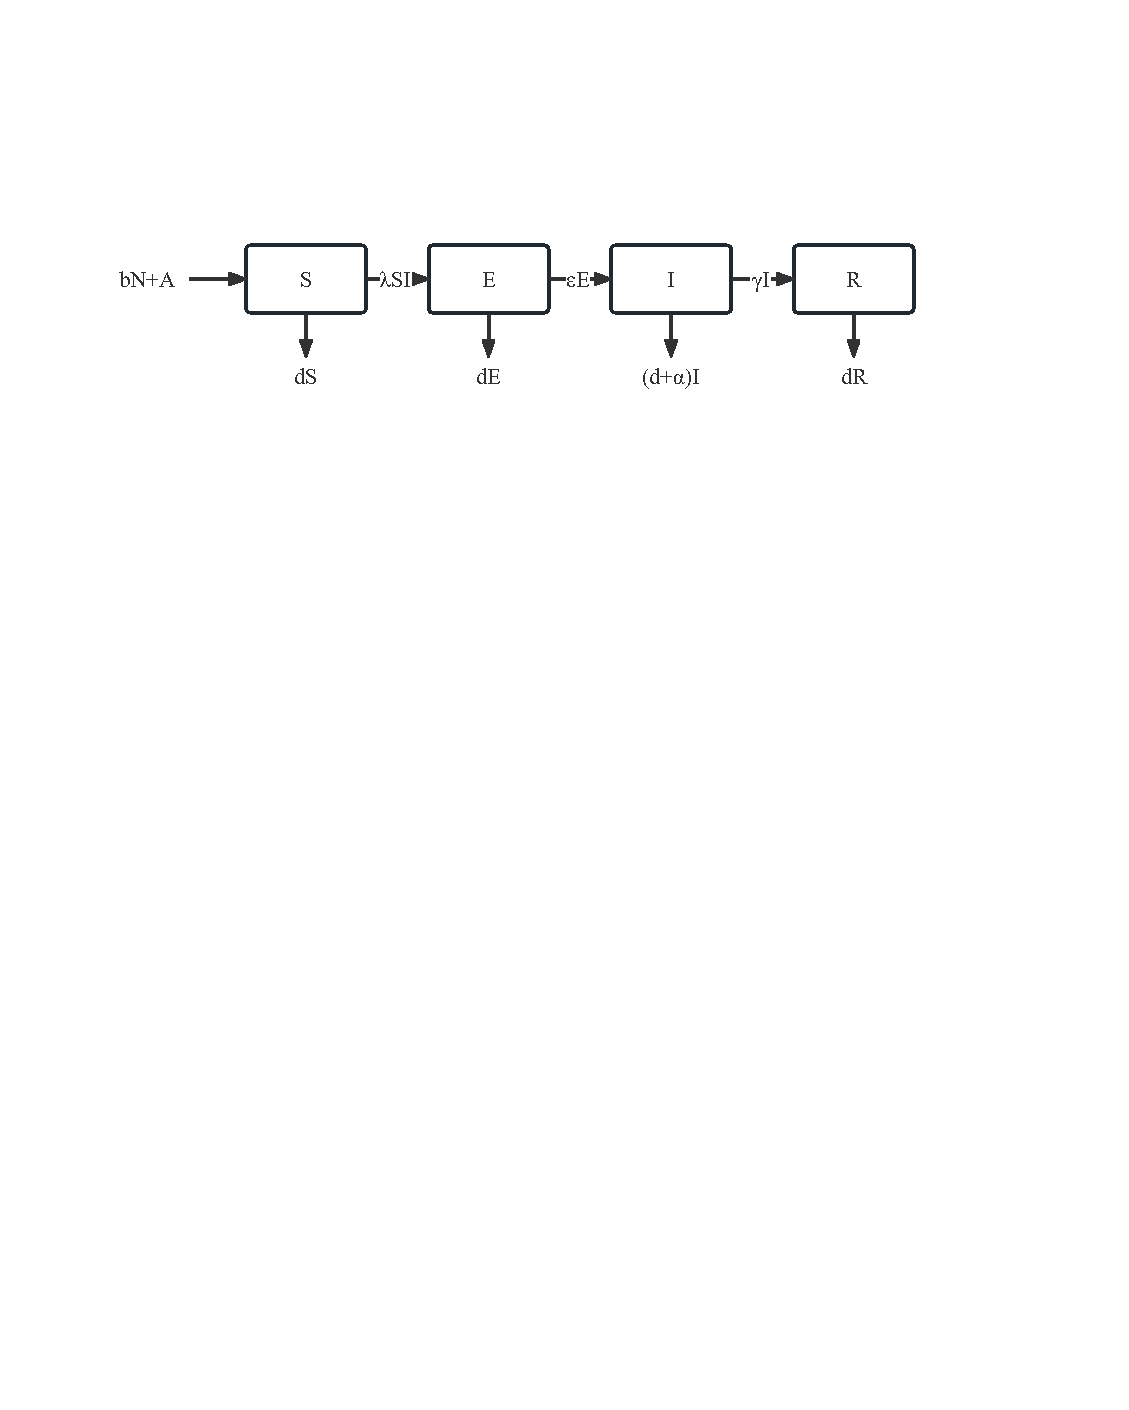
\includegraphics{image/NewSEIR}
    \caption{具有常数移民出生的SEIR模型}
    \label{img:NewSEIR}
\end{figure} 

根据框图结构,可以写出如下微分方程组

\begin{gather}
    \left\{
    \begin{aligned}
    \frac{dS}{dt} & =  bN + A-dS-\frac{\lambda IS}{N} \\
    \frac{dE}{dt} & =  \frac{\lambda SI}{N} - (\varepsilon +d)E\\
    \frac{dI}{dt} & =  \varepsilon E - (\gamma +\alpha +d)I\\
    \frac{dR}{dt} & =  \gamma I - dR \\
    \end{aligned}
    \right.
    \label{equal:NewSEIR}
\end{gather}
其中$b$为出生率,$d$为死亡率,$A$为迁移人数,$\lambda$为有效接触率,$\varepsilon$为发病率,$\alpha$为病死率,$\gamma$为治愈率。

在实际防控中,人口变化因素的影响是不可忽略的,如移民可能会带来疫情的跨区域传播,出生则可能导致病毒在人群中持续存在,死亡可能会导致病例数下降等等,因此,将这些因素考虑进模型中,可以更好地指导防控措施的制定和实施。将移民、出生和死亡等因素纳入SEIR模型中,可以更加真实地反映传染病的传播和演化过程,提高预测和指导防控的准确性和有效性。
\subsubsection{模型分析}
总人口$N(t)=S(t)+E(t)+I(t)+R(t)$满足方程

\begin{gather}
    N'=(b-d)N-\alpha I+A
    \label{equal:N'}
\end{gather}

做归一化变换

$$s=\frac{S}{N}, e=\frac{E}{N}, i=\frac{I}{N}, r=\frac{R}{N}, $$
因为$s+e+i+r=1$,且只有最后一个方程含$R$,故只需要考虑(\ref{equal:NewSEIR})的前三个方程

\begin{gather}
    \left\{
    \begin{aligned}
    \frac{ds}{dt} & =  b + A'-d-\lambda is \\
    \frac{de}{dt} & =  \lambda si - (\varepsilon +d)e\\
    \frac{di}{dt} & =  \varepsilon e - (\gamma +\alpha +d)i\\
    \end{aligned}
    \right.
    \label{equal:seir}
\end{gather}

方程(\ref{equal:seir})的可行域

$$D={(s,e,i)\in R^3_+|0\leqslant s+e+i\leqslant 1}.$$
容易验证$D$是系统(\ref{equal:seir})的一个正向不变集,系统(\ref{equal:seir})的修正再生数为

$$\theta =\frac{\lambda \varepsilon A}{(b+\varepsilon)(\gamma +\alpha +b) }$$
方程(\ref{equal:seir})总存在无病平衡点$P_0(1,0,0)$,且当$\theta>1$时,有唯一的正平衡点$p^*(s^*,e^*,i^*)$。

\subsection{通用微分方程}
最近几年机器学习发展迅速,在耦合微分方程和深度神经网络方面有了重大的进展,但是像通用微分方程\ucite{2020Universal}这样的深度学习方法在流行病控制、流行病预测和流行病模型研究方面的应用还没有得到足够的重视\ucite{Song2022ESTIMATINGTR}。这可能是因为这些领域需要研究人员具有强大的流行病学、深度学习、微分编程和科学计算的基本理解。为了填补这一空白,我们引入了通用微分方程,利用其来解决最优流行病控制问题,从而推动了这一领域的发展。通用微分方程具有广泛的适用性和灵活性,可以有效地解决不同类型的流行病动力学问题,提高流行病模型的准确性和可解释性。这种方法不仅可以加深我们对流行病传播和控制的理解,还可以为公共卫生决策提供有力的支持。

在介绍通用微分方程(Universal Differential Equation)之前,我们先来谈谈神经微分方程(Neural Differential Equation)\ucite{2018Neural}。神经微分方程可以看作是通用微分方程的一个特例,它启发了通用微分方程的发展。神经微分方程是一类具有特定形式的初值问题,它们将微分方程和神经网络结合起来,利用神经网络来近似微分方程的解。通过在微分方程中引入神经网络的概念,可以将微分方程的求解转化为神经网络的优化问题,从而实现更加高效、准确的求解。通用微分方程则是更为广泛的一类微分方程形式,不仅包括神经微分方程,还包括许多其他类型的微分方程。通过使用通用微分方程,我们可以更加灵活地建立流行病动力学模型,实现更加准确、可靠的预测和控制。同时,通用微分方程还具有很好的可解释性,能够提高我们对流行病学问题的理解。神经微分方程是具有以下形式的初值问题:

\begin{gather}
    u'=N_\theta(u,t)
\end{gather}
神经微分方程可以看作是UDE的一种特例,它是一种基于微分方程数值方案重新设计的时序神经网络,可以被视为一种无限深或连续深的类ResNet深度学习模型。神经微分方程利用嵌入式神经网络作为通用逼近器,能够学习逼近任何微分方程的规律性。然而,神经微分方程仍然是一种数据驱动的方法,缺乏已知的知识或机制。

相比之下,通用微分方程扩展了数据驱动的神经 ODE 方法,能够直接利用机械建模和通用逼近器。通用微分方程是一个初值问题,通过一个深度神经网络 $N_\theta$,以接收 $[u, t]$ 作为输入,其中 $\theta$ 是权重参数向量。由于深度神经网络是通用逼近器,因此UDE可以被用来解决多种微分方程问题,包括流行病动力学中的SEIR模型。UDE具有较高的灵活性和适应性,同时也提供了一种强大的工具来结合领域知识和数据驱动建模。 UDE 是初值问题如下的微分方程组:

\begin{gather}
    u'=f_{\theta_2}(u,t,N_{\theta_1}(u,t))
\end{gather}

这里 f 是基于知识的或已知的机制模型,$N_{\theta_1}(u,t)$ 表示缺失或未知项,θ1 和 θ2 分别是已知机制和神经网络的参数,可以同时估计。相比于黑盒深度神经网络或神经微分方程,UDE在物理、化学、生态学或流行病学等领域中,能够更好地利用已知机制,并且对于少量的样本数据也具有较好的泛化能力\ucite{2020Universal}。因此,UDE有望成为未来在科学领域中的一种重要建模和预测方法。

\subsubsection{嵌入ODE的神经网络}
通用微分方程(Universal Differential Equation,简称 UDE)是一种嵌入了通用逼近器的特殊微分方程。这里的“通用逼近器”可以是各种数学逼近方法,如神经网络、高斯过程、决策树、切比雪夫多项式、傅立叶级数等。在本文中,我们以神经网络作为通用逼近器。通过将通用逼近器嵌入微分方程中,UDE 将微分方程与深度学习结合起来,可以高效地推断原始部分观测数据,并以可微分和完全观测的拟合数据形式进行表示。此外,UDE 也可以高效地利用时间和数据来解决优化问题。在接下来的内容中,我们将介绍深度神经网络和通用微分方程,并阐述如何通过训练嵌入神经网络的参数来优化问题。值得注意的是,UDE 作为一种基于知识的、数据驱动的方法,不仅具有良好的可解释性,而且可以利用已知的物理、化学、生态学或流行病学机制来提高模型的泛化能力。

考虑由Betts\ucite{2010Practical}和Lenhart等\ucite{2007Optimal}提出的如下形式的最优控制问题:

\begin{gather}
    \left\{\begin{aligned}
        \min _{u(\cdot), x(\cdot)} J & =\int_{0}^{T} g(x, u, t) d t+\phi(x(T), T) \\
        \text { s.t. } \frac{\mathrm{d} x}{\mathrm{dt}} & =f(x, u, t), x(0)=x_{0}, t \in[0, T], \\
        u_{i}(t) & \in\left[a_{i}, b_{i}\right], 1 \leq i \leq m, t \in[0, T],
        \end{aligned}\right.
        \label{equal:control}
\end{gather}
其中函数$u: \mathbb{R} \rightarrow \mathbb{R}^{m}, f: \mathbb{R}^{n} \times \mathbb{R}^{m} \times \mathbb{R} \rightarrow \mathbb{R}^{n}, g: \mathbb{R}^{n} \times \mathbb{R}^{m} \times \mathbb{R} \rightarrow \mathbb{R},\phi : \mathbb{R}^{n} \times \mathbb{R} \rightarrow \mathbb{R}$为连续可微的,而$u(t)$代表神经网络,$\theta$为神经网络中的参数。

\begin{gather}
    u(t)=N_\theta (t,x)
\end{gather}
神经网络接受输入 $t$ 和 $x$,用于解决最优控制问题。最优控制是一个广义的概念,涉及到许多现实世界中的问题。深度学习模型的训练本质上也是为了解决最优控制问题。许多数据驱动的流行病问题可以被视为或转化为最优控制问题。我们通常使用某种损失函数来评估模型的拟合效果。该损失函数可能是基于真实数据与模型预测之间的误差,或者是基于一组特定的目标来衡量。通过优化损失函数,我们可以调整神经网络的参数,以便找到最优解来解决所面临的最优控制问题。一般使用某种损失函数来衡量模型拟合效果的好坏:

\begin{gather}
    Loss=\sum_{n = 1}^{\infty} ||\widetilde{g}_\theta(x(t_i))-y_i|| 
    \label{equal:loss}
\end{gather}
其中$\widetilde{g}_\theta$为在参数$\theta $下的输出函数,$D\{(x_i,y_i),i\in T\}$为输入数据,则最优控制问题(\ref{equal:control})变为如下形式:

\begin{gather}
    \left\{\begin{aligned}
        \min _{\theta} J & =Loss(D,\widetilde{g}_\theta) \\
        \text { s.t. } \frac{\mathrm{d} x}{\mathrm{dt}} & =f(x, N_\theta (t,x), t), x(0)=x_{0}, t \in[0, T], \\
        \end{aligned}\right.
\end{gather}

相比于其他基于深度学习的常微分方程求解方法,通用微分方程是数据驱动的。它基于知识的方法,比黑盒深度神经网络或神经微分方程具有更强的可解释性,因为它们保留了物理、化学、生态学或流行病学中的已知机制。 通用微分方程被证明是一种具有良好泛化能力的方法,可以用较少的样本数据进行训练\ucite{2020Universal}。

\subsubsection{具有约束方程的反向传播}
现在考虑微分方程组(\ref{equal:control})的参数优化问题,为了使用反向传播算法对其进行优化,首先要求得目标函数对参数的偏导数$\frac{\partial J}{\partial \theta}$。首先引入拉格朗日乘数$\lambda$:

\begin{gather}
    J(\theta)=\int^T_0 g(x,u,t)dt+\int^T_0 \lambda(m(x,\theta,t)-f(x,p,t))dt
\end{gather}

因为$x'=f(x,p,t)$,有
\begin{gather}
    \begin{aligned}
        \frac{dJ(\theta)}{d\theta} &=\int^T_0 g_xx_\theta +\lambda'(t)x_\theta +\lambda(t)(m_xx_\theta+m_\theta) dt +\lambda(T)|_{t=T}\\
        &=\int^T_0 [\lambda'(t)+g_x+m_x\lambda(t)]x_\theta dt+\int^T_0 \lambda(t)m_\theta dt -\lambda(T)x_\theta|_{t=T}
    \end{aligned}
\end{gather}
令

\begin{gather}
    \lambda'(t)=-g_x-m_x\lambda(t),\lambda(T)=0
\end{gather}
则得到
\begin{gather}
    \frac{dJ}{d\theta}=\int^T_0 \lambda(t)m_\theta dt
\end{gather}

于是将原优化问题(\ref{equal:control})转化为

\begin{gather}
    \left\{\begin{aligned}
        \frac{dJ}{d\theta}&=\int^T_0 \lambda(t)m_\theta dt,\\
        \lambda' (t)&=-g_x-m_x\lambda(t),\lambda(T)=0,\\
        x'&=m(x,\theta,t),x(0)=x_0.
        \end{aligned}\right.
    \label{equal:final}
\end{gather}

通过上述过程,我们不再需要解决$\theta$维的常微分方程组来解决优化问题(\ref{equal:control})。相反,我们只需要解决与$\theta$无关的维度为$2n$的常微分方程组(\ref{equal:final}),这使得我们可以将大规模神经网络与微分方程相结合。神经网络通常具有巨大的参数量,因此解决如此高维度的常微分方程组将需要大量的计算时间和资源。为了解决这个问题,我们可以采用两种方法对$2n$维常微分方程组进行数值求解。一种方法是连续伴随方法,也称为微分然后离散化方法,它通过数值离散化来求解常微分方程组(\ref{equal:final})中的伴随微分方程(λ(t))\ucite{2014FATODE}。另一种方法是离散伴随灵敏度法,也称为先离散后微分法,它首先对正向系统(x(t))进行数值逼近,然后得到(x(t))的离散系统的伴随\ucite{2018A}。这些方法的使用使得我们可以更有效地解决复杂的优化问题,为数据驱动的流行病问题提供更加准确和可靠的解决方案。
\subsubsection{通用SEIR方程}

在具有移民和出生的 SEIR 模型(\ref{equal:NewSEIR})中,可以再次添加三个变量,N:总人数;D:死亡数;C:累计病例。这于是模型变为如下形式:

\begin{gather}
    \left\{
    \begin{aligned}
    \frac{dS}{dt} & =  bN + A-dS-\frac{\lambda IS}{N} \\
    \frac{dE}{dt} & =  \frac{\lambda SI}{N} - (\varepsilon +d)E\\
    \frac{dI}{dt} & =  \varepsilon E - (\gamma +\alpha +d)I\\
    \frac{dR}{dt} & =  \gamma I - dR \\
    \frac{dN}{dt} & = (b-d)N+A-\alpha I \\
    \frac{dD}{dt} & = dN+\alpha I \\
    \frac{dC}{dt} & = \frac{\lambda IS}{N}
    \end{aligned}
    \right.
    \label{equal:USEIR}
\end{gather}

其中$b,A,d,\lambda,\varepsilon,\alpha,\gamma$为方程的参数,可以用神经网络$N_\theta(u,t)$替代,$N_\theta(u,t): \mathbb{R}^m \rightarrow \mathbb{R}^{n}$。(\ref{equal:USEIR})的前四个方程中不含$N,D,C$,所以在(3.1.2)节中分析得到的微分方程组的性质仍然适用。

在疫情流行期间,易感者数(S)、潜伏者人数(E)是较难统计的,而患病人数(I)、死亡人数(D)、累计感染人数(C)、总人口(N)是比较容易通过统计和筛查得到的;而这些统计数据之间又有部分具有一定的相关性,所以一般选择患病人数(I)、死亡人数(D)、累计感染人数(C)、总人口(N)中的一部分变量作为神经网络的输入变量。在疫情控制和防控策略制定中,有效接触率($\lambda $)、基本再生数($R_0$)、平均患病周期($\gamma$)、疾病致死率($\alpha$)是了解和分析疫情传播规律,制定相应的控制措施的主要依据之一;相对于传染病的流行时间,一个地区的出生率(b)、自然死亡率(d)变化幅度不大,可以近似地认为是一个相对于时间不变的常数;而迁入率和迁出率是可以通过制定政策、控制交通等方式控制的。所以一般选择有效接触率($\lambda $)、基本再生数($R_0$)、平均患病周期($\gamma$)、疾病致死率($\alpha$)作为神经网络的输出变量。

相比于黑盒深度学习模型,通用SEIR方程(USEIR)保留了流行病动力学中的已知机制,保留了SEIR模型的舱室结构和各个舱室之间的转换关系,因此更容易解释模型的预测结果;同时在流行病学中,通常只有有限的数据可用于训练模型,而UDE 被证明是一种具有良好泛化能力的方法,可以使用较少的样本数据进行训练,因此 USEIR 可以帮助提高模型的预测准确性;由于 USEIR 能够将已知的机制和数据驱动的方法相结合,因此可以获得更高的预测精度;由于 USEIR 可以高效地推断原始的部分观测数据,因此可以获得可微分和完全观测的拟合数据,所有这些都以时间和数据高效的方式进行,这使得 USEIR 在实时决策中具有优势。下面一章将通过数值模拟和对美国加利福尼亚州的COVID-19疫情数据的拟合和预测说明USEIR的优越性。

\newpage
\section{实验与分析}
本章中,我们使用USEIRE方法基于数值模拟的传染病模型和加利福尼亚州第一波COVID-19病例数据来估计有效再生数$R_0$。结果表明,USEIRE可以很好地拟合数据,深度神经网络可以很好地表示$R_0$。本章的所有深度学习方法和数据处理均在开源的Julia语言1.8.5中实现,在装有1.60GHz i5-8265U CPU和16G RAM的笔记本电脑上使用Ubuntu操作系统进行了实验。

本章使用的网络结构为模型(\ref{equal:USEIR}),其中神经网络$N_\theta(u,t)$为$m\times 64\times 64\times n$的全连接网络,并以 tanh 作为激活函数。其中$m,n$分别为输入参数量和输出参数量,在不同的任务中会对不同的参数进行预测、拟合。
\subsection{数值模拟}
首先使用数值求解器对模型(\ref{equal:USEIR}),其中参数都为常数,生成30个时间单位的数据。使用USEIR模型对生成的数据进行预测,其中损失函数为(\ref{equal:loss}),神经网路的输入为$S,I,D$,需要预测的参数为$\lambda , \alpha, \gamma$ 则整个预测模型可以写为如下形式:

\begin{gather}
    \left\{
    \begin{aligned}
    & \mathop{max}\limits_\theta \sum_{n = 1}^{\infty} ||\widetilde{g}_\theta(x(t_i))-y_i||  \\
    \frac{dS}{dt} & =  bN + A-dS-\frac{\lambda IS}{N} \\
    \frac{dE}{dt} & =  \frac{\lambda SI}{N} - (\varepsilon +d)E\\
    \frac{dI}{dt} & =  \varepsilon E - (\gamma +\alpha +d)I\\
    \frac{dR}{dt} & =  \gamma I - dR \\
    \frac{dN}{dt} & = (b-d)N+A-\alpha I \\
    \frac{dD}{dt} & = dN+\alpha I \\
    \frac{dC}{dt} & = \frac{\lambda IS}{N} \\
    \lambda , \alpha, \gamma & ={NN}_\theta (S,I,R)
    \end{aligned}
    \right.
    \label{equal:1}
\end{gather}

选取前10个时间单位的数据添加0.01强度的高斯噪声进行训练,选取ADAM优化器设置学习率为0.01,训练100次;再使用BFGS优化器在之前训练的最优结果上再次训练,初始步长为0.01,在损失函数接近最小值时停止训练,模型迭代的过程如下图:

可以看出

\subsection{拟合与预测}
流行病是由自然界中的病原体引起的,具有复杂性和不确定性,因为它们受到多种因素的影响,如病原体的属性、宿主的免疫力、人群的行为、社会环境等,而且在传播过程中存在不可预测的变化和干扰,如变异株的出现、政策干预等。除此之外,流行病在不同的时间和地点表现出不同的特征,因此需要对不同的流行病进行不同的处理,而模型是基于数学公式和假设来预测疾病传播的。为了测试USEIR模型对于现实世界中流行病的拟合和预测能力,本文选取美国佛罗里达州2021年的第一波COVID-19疫情数据进行测试。

\subsubsection{参数拟合}
\subsubsection{数据预测}
\subsubsection{对比实验}
\subsection{结果分析}

\newpage
\section{结论}

\section*{致谢}
\addcontentsline{toc}{section}{致谢}